%Pretreatment========================================================================================
\documentclass[12pt]{article}
\usepackage{lingmacros}
\usepackage{tree-dvips}
\usepackage{graphicx}
\usepackage{hyperref}
\usepackage{amsmath}
\usepackage{amssymb}
\usepackage{multicol}
\usepackage{geometry}
\usepackage{cite}
\usepackage[amsmath,thmmarks]{ntheorem}
\usepackage{algpseudocode}
\usepackage{algorithm}
\usepackage{listings} 
\usepackage{verbatim}
\usepackage{subfigure}
\usepackage{appendix}  
\usepackage{color}
%\usepackage{subcaption}


\theoremstyle{plain}
\theoremseparator{\hspace{1em}} \theoremnumbering{arabic}
\theoremsymbol{}
\newtheorem{theorem}{\textbf{Theorem}}[section]
\newtheorem{definition}{\textbf{Definition}}[section]
\newtheorem{lemma}{\textbf{Lemma}}[section]
\newtheorem{proof}{\textit{PROOF}}[section]
\newtheorem{example}{\textbf{E x a m p l e}}[section]
\newtheorem{solution}{\textit{SOLUTION}}[section]

\geometry{left=2cm,right=2cm,top=3cm,bottom=2cm}
\title{[Note] Chaos: An Introduction to Dynamical Systems}
\author{}
\date{\today}

\begin{document}
\maketitle

{
\begin{center}
\LARGE \textbf{Problem in discrete-time system}
\end{center}
}
\section{One-Dimension Maps}

\begin{definition}\textbf{n-order differentiable function, Smooth function, Map}
\\\noindent Consider an open set $E$ and $n \in \mathcal N$, called 
$$
C^n(E) = \{f \in C(E) | \forall \alpha \text{ s.t. } |\alpha| \leq n, D^\alpha f \in C(E)\}
$$
is n-order differentiable function set of $E$, where $C(E)$ is continuous function on $E$.
\\\noindent If $f$ on domian $E$ have infinity-order derivative, or $f \in C^\infty(E)$, then called $f$ \textbf{smooth function}.
\\\noindent If the function $f$ have same domain and range, then called $f$ is a \textbf{map}.
\end{definition}

{\color{red} The fucntion in this book will be a smooth function if we not emphasize.}

\begin{definition}\textbf{Orbit, initial value, fixed point}
\\\noindent Consider a map $f: X \rightarrow X$, $x$ is a point in $X$ then 
\\\noindent Called \textbf{orbit} of $x$ is a set of point 
$$
\text{Orbit}(X) = \{x, f(x), f^2(x), \ldots f^n(x), \ldots\}
$$
, where $f^n(x) = f(f(\ldots f(x))) = (f\circ f \circ f \circ \ldots \circ f)(x)$.
\\\noindent The starting point of $x$ for a orbit called the \textbf{initial value}.
\\\noindent If the point $p$ s.t. $f(p) = p$, then called $p$ as fixed point.
\end{definition}

OK, and now we consider two dynamical systems, with a input $x$, the system will always return to $f(x) = 2x$ and $g(x) = 2x(1-x)$. And then the output will become the input value and etc. During this looping, it is simple to find the orbit of a certain initial value.


\begin{table}[H]
\centering  
\caption{Comparison of exponential growth and logistic growth}  
\begin{tabular}{|c||c|c|c|c|c|c|c|c|c|c|}
\hline
f & init & 1 & 2 & 3 & 4 & 5 & 6 & 7 & 8 & 9 \\
\hline
\hline
$f(x)$ & 0.01 & 0.02   & 0.04   & 0.08   & 0.16   & 0.32     & 0.64        & 1.28  & 2.56  & 5.12  \\
\hline
$f(x)$ & 0.01 & 0.0198 & 0.0388 & 0.0746 & 0.138  & 0.268    & 0.362       & 0.462 & 0.497 & 0.499 \\
\hline
$g(x)$ & 0.5  & 0.5    & 0.5    & 0.5    & 0.5    & 0.5      & 0.5         & 0.5   & 0.5   & 0.5   \\
\hline
$g(x)$ & 0.8  & 0.32   & 0.435  & 0.492  & 0.499  & 0.5      & 0.5         & 0.5   & 0.5   & 0.5   \\
\hline
$g(x)$ & 1.2  & -0.48  & -1.42  & -6.87  & -108.4 & -23716.9 & -1125030476 & -inf  & -inf  & -inf  \\
\hline
\end{tabular}  
\end{table}  

We found that in the model of $f$, the result is growth as exponential function and we called that exponential growth. Also, when intial value $x \in [0, 1]$, with iteration, the result have limition of 0.5 and we called these model as logistic growth.

In this section, we will mainly focus on these kind of dynamical system, obviously, the iteration processing of model are discrete, we also called these dynamical system models as \textbf{maps}.






\subsection{Cobweb plot, stability and }
To analysis a maps, the basic method is based on cobweb plot. Fig \ref{cobweb-plow-1} showed a method to analysis a dynamical system with a certain iteration principle. 
\begin{figure}[H]
\begin{center}
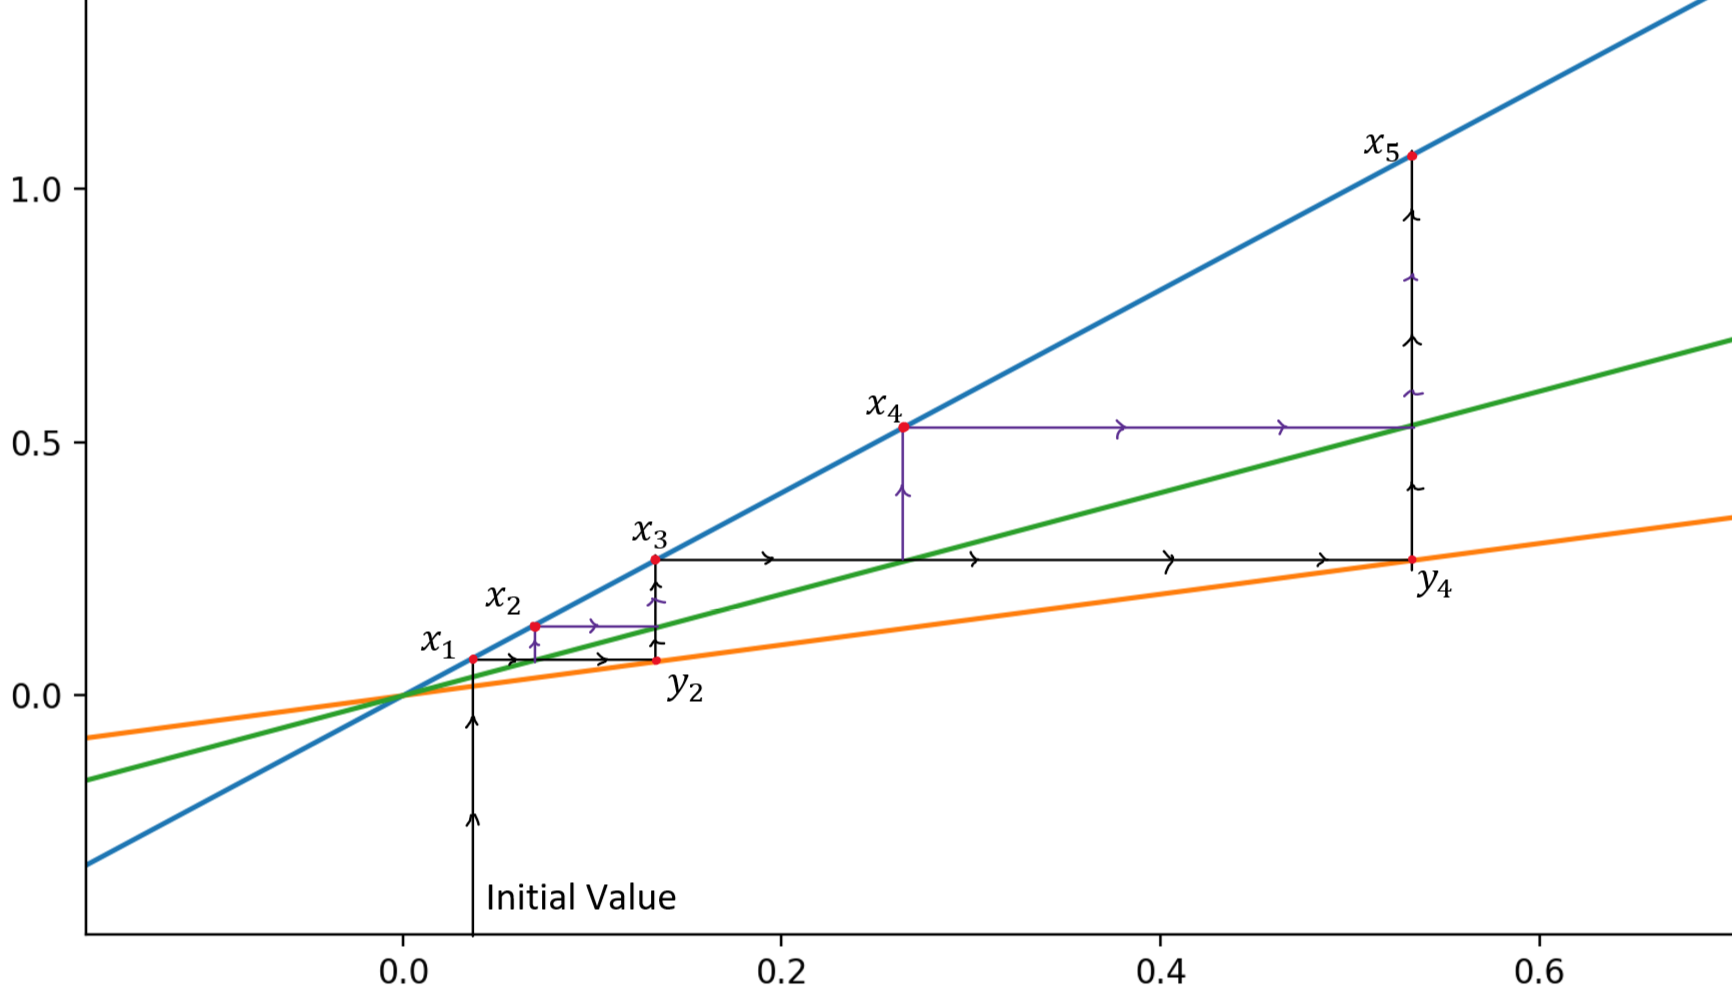
\includegraphics[width=0.6\textwidth]{figure/section1/cobweb-plot.png} \\
\caption{An example of cobweb plot and basic principle}\label{cobweb-plow-1}
\end{center}
\end{figure}

In every iteration, the independent and dependent variable exchanged their location and we can found a group of $\{x_1, y_2, x_3, y_4, \ldots\}$ as orbit of initial value. Or, with the symmetric line $y = x$, it is simple to symmetric all black line to purple line and we can build a cobweb plot with origin image and $y = x$ to find a group of $\{x_1, x_2, \ldots\}$ as orbit from the initial value.

Before we discuss the different of fixed point, it is necessary to review some basic definitions.

\begin{definition}\textbf{$\varepsilon$ Neighbourhood}
\\\noindent In a metric space $X$, an $\varepsilon$ neighbourhood $N_\varepsilon(p)$ of point $p$ is defined 
$$
N_\varepsilon(p) = \{x \in X | d(x, p) < \varepsilon\}
$$
where $d(x, p)$ is the distance bewteen point $p$ and $x$. Also, in a $R^1$ space, the $\varepsilon$ Neighbourhood is give by
$$
N_\varepsilon(p) = \{x \in R | |x-p| < \varepsilon\}
$$
\end{definition}


\newpage

\begin{figure}[H]
\begin{minipage}[c][0.6\width]{
   0.5\textwidth}
   \centering
   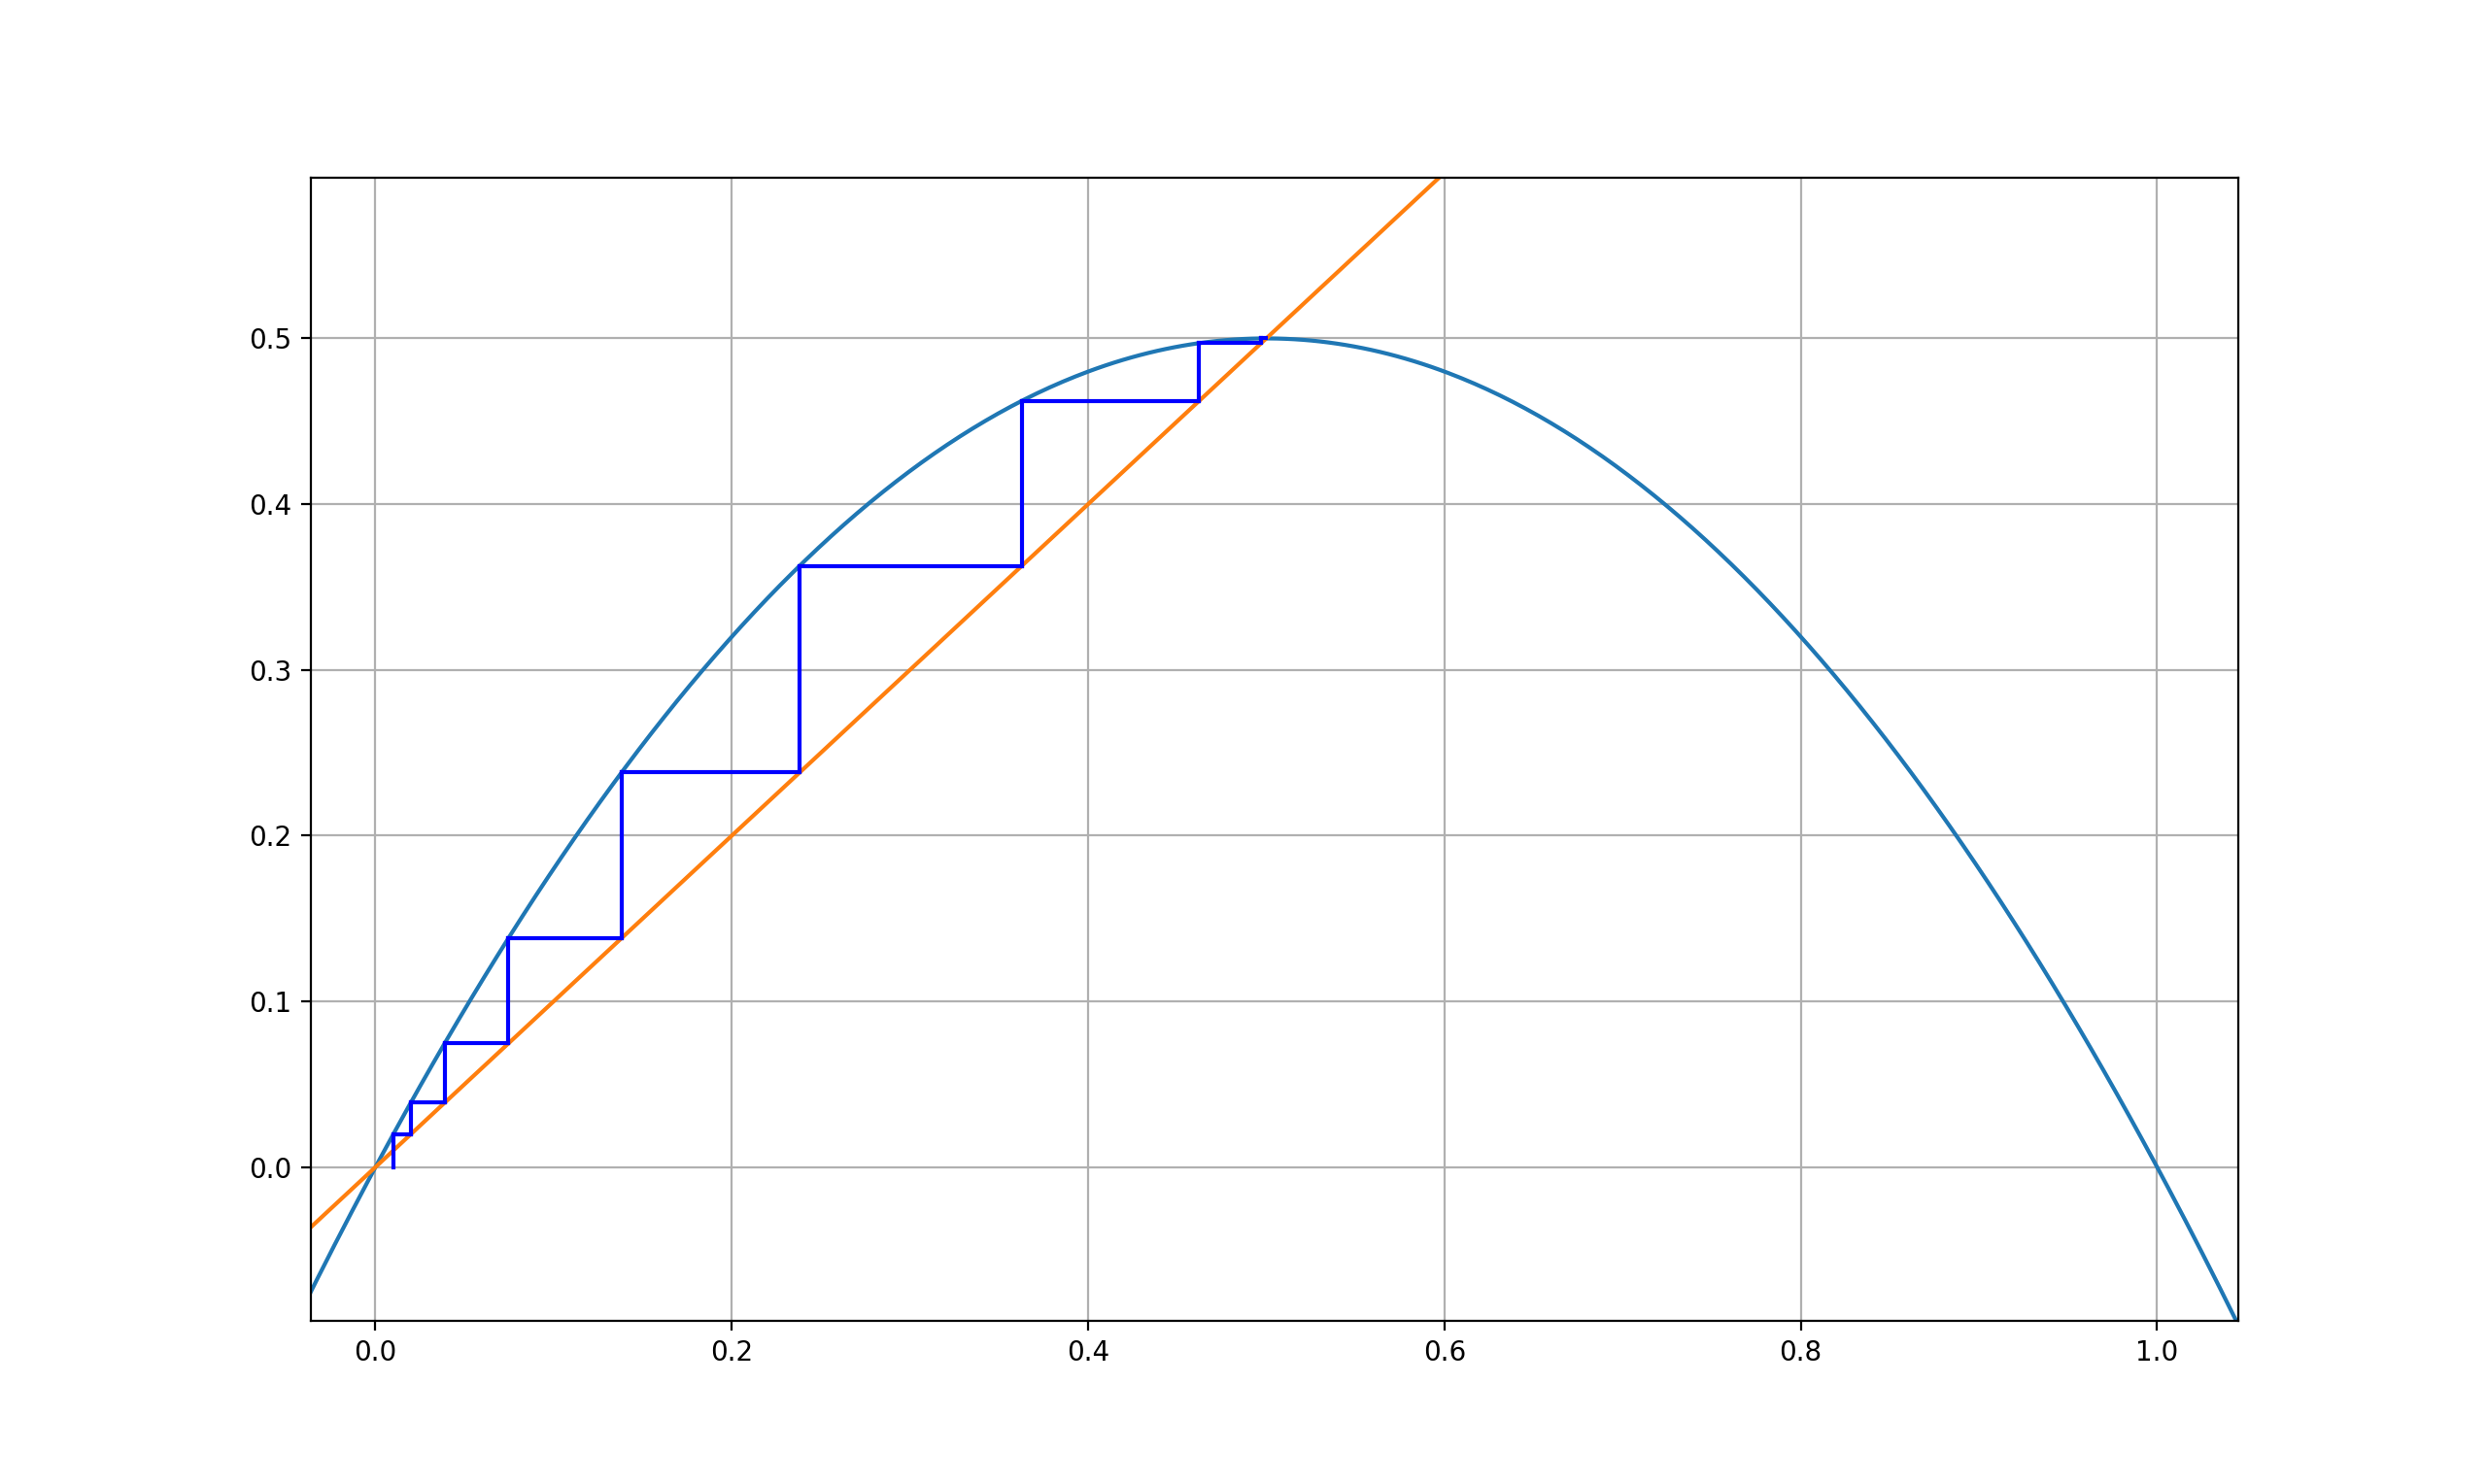
\includegraphics[width=1\textwidth]{figure/section1/cb01.png}
\end{minipage}
\begin{minipage}[c][0.6\width]{
   0.5\textwidth}
   \centering
   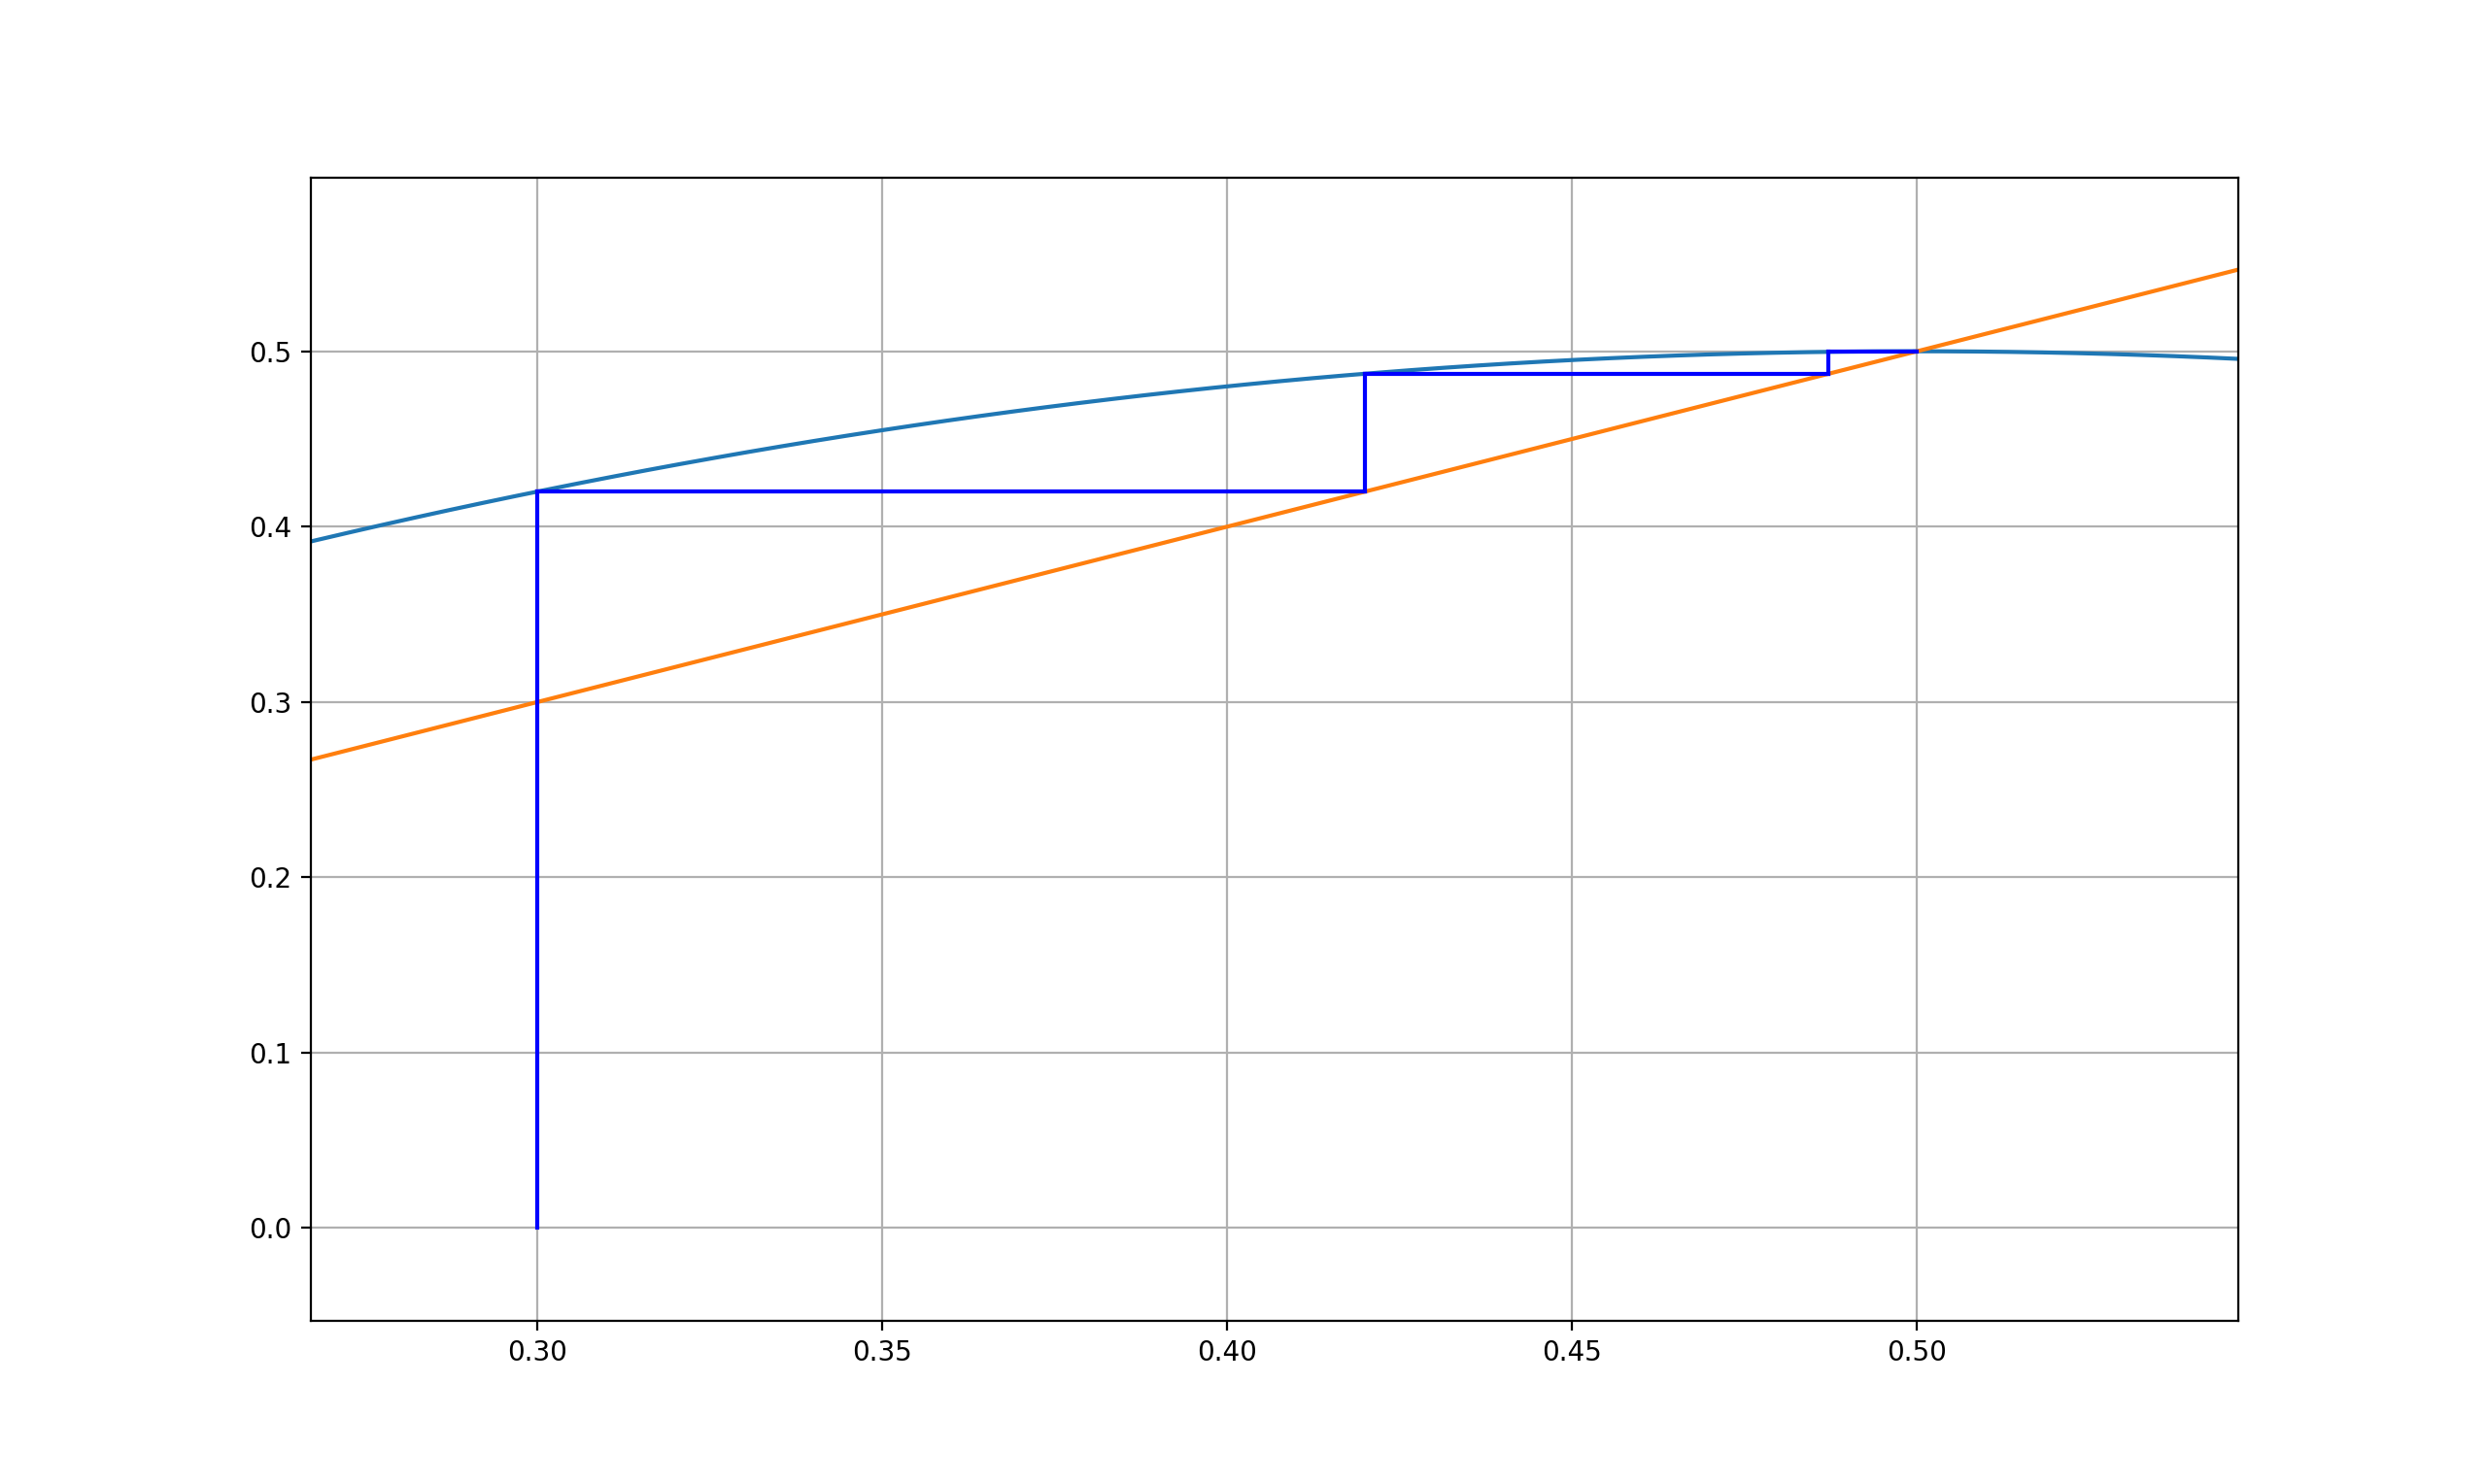
\includegraphics[width=1\textwidth]{figure/section1/cb02.png}
\end{minipage}
\begin{minipage}[c][0.6\width]{
   0.5\textwidth}
   \centering
   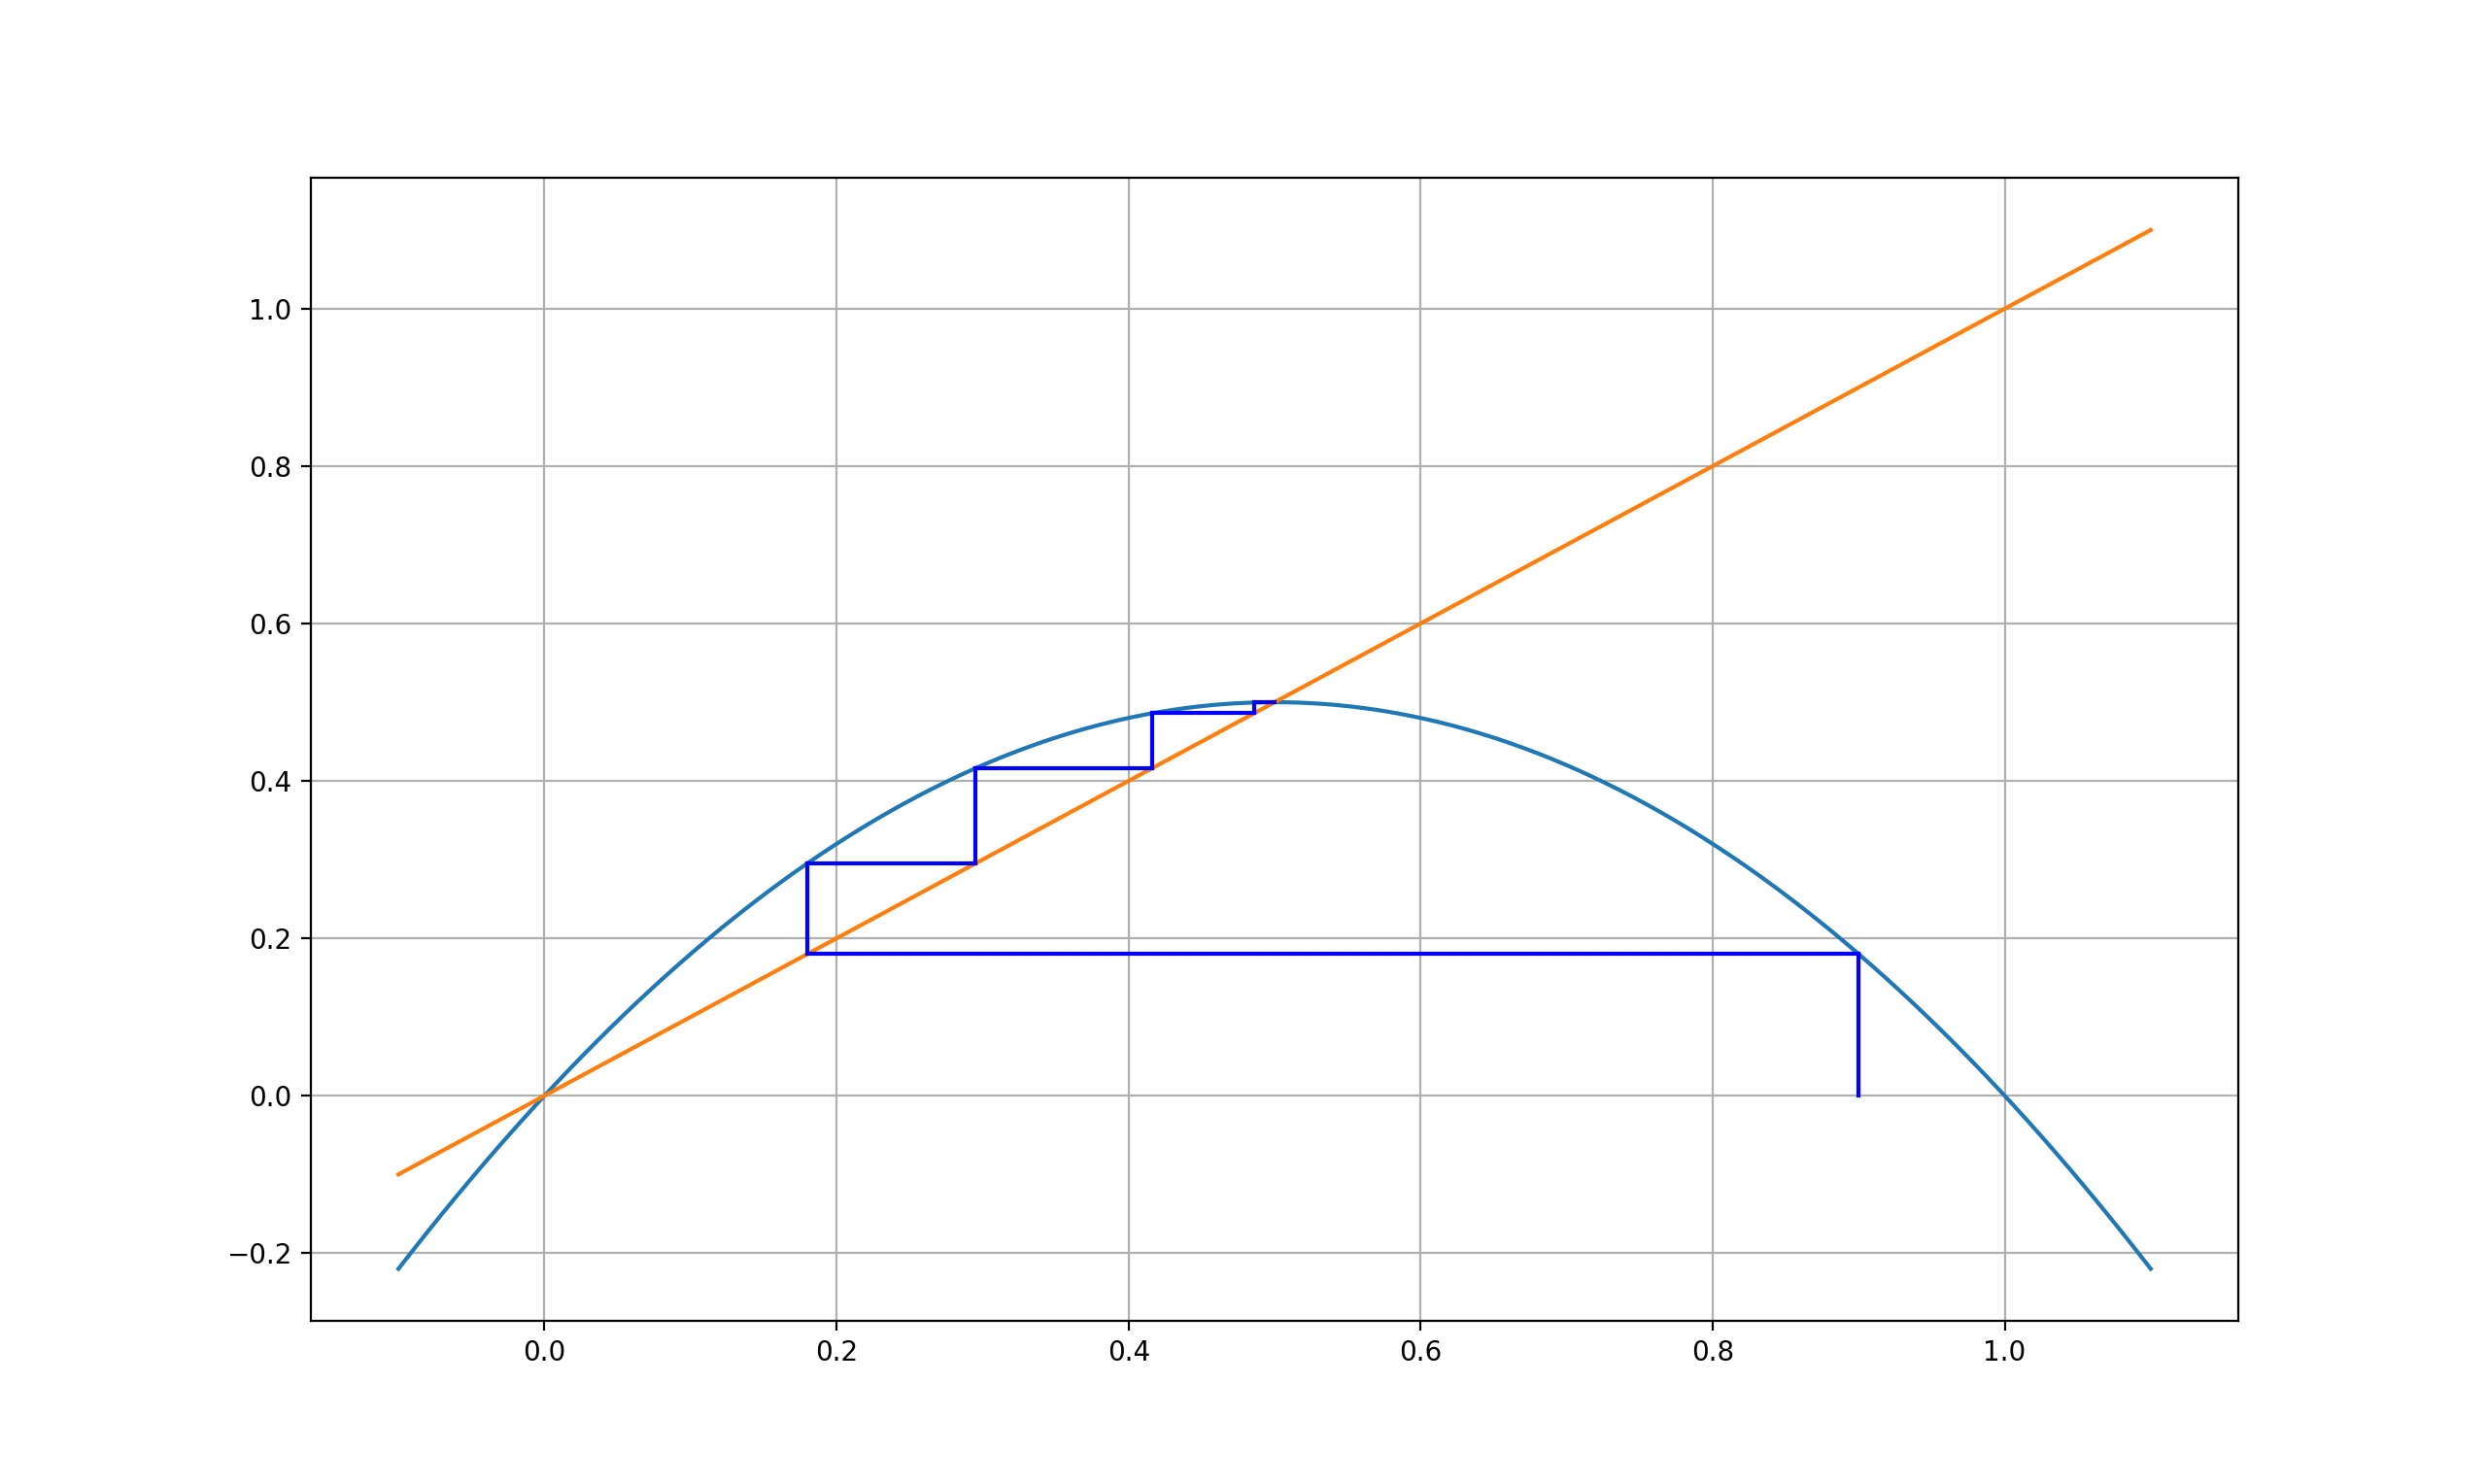
\includegraphics[width=1\textwidth]{figure/section1/cb03.png}
\end{minipage}
\begin{minipage}[c][0.6\width]{
   0.5\textwidth}
   \centering
   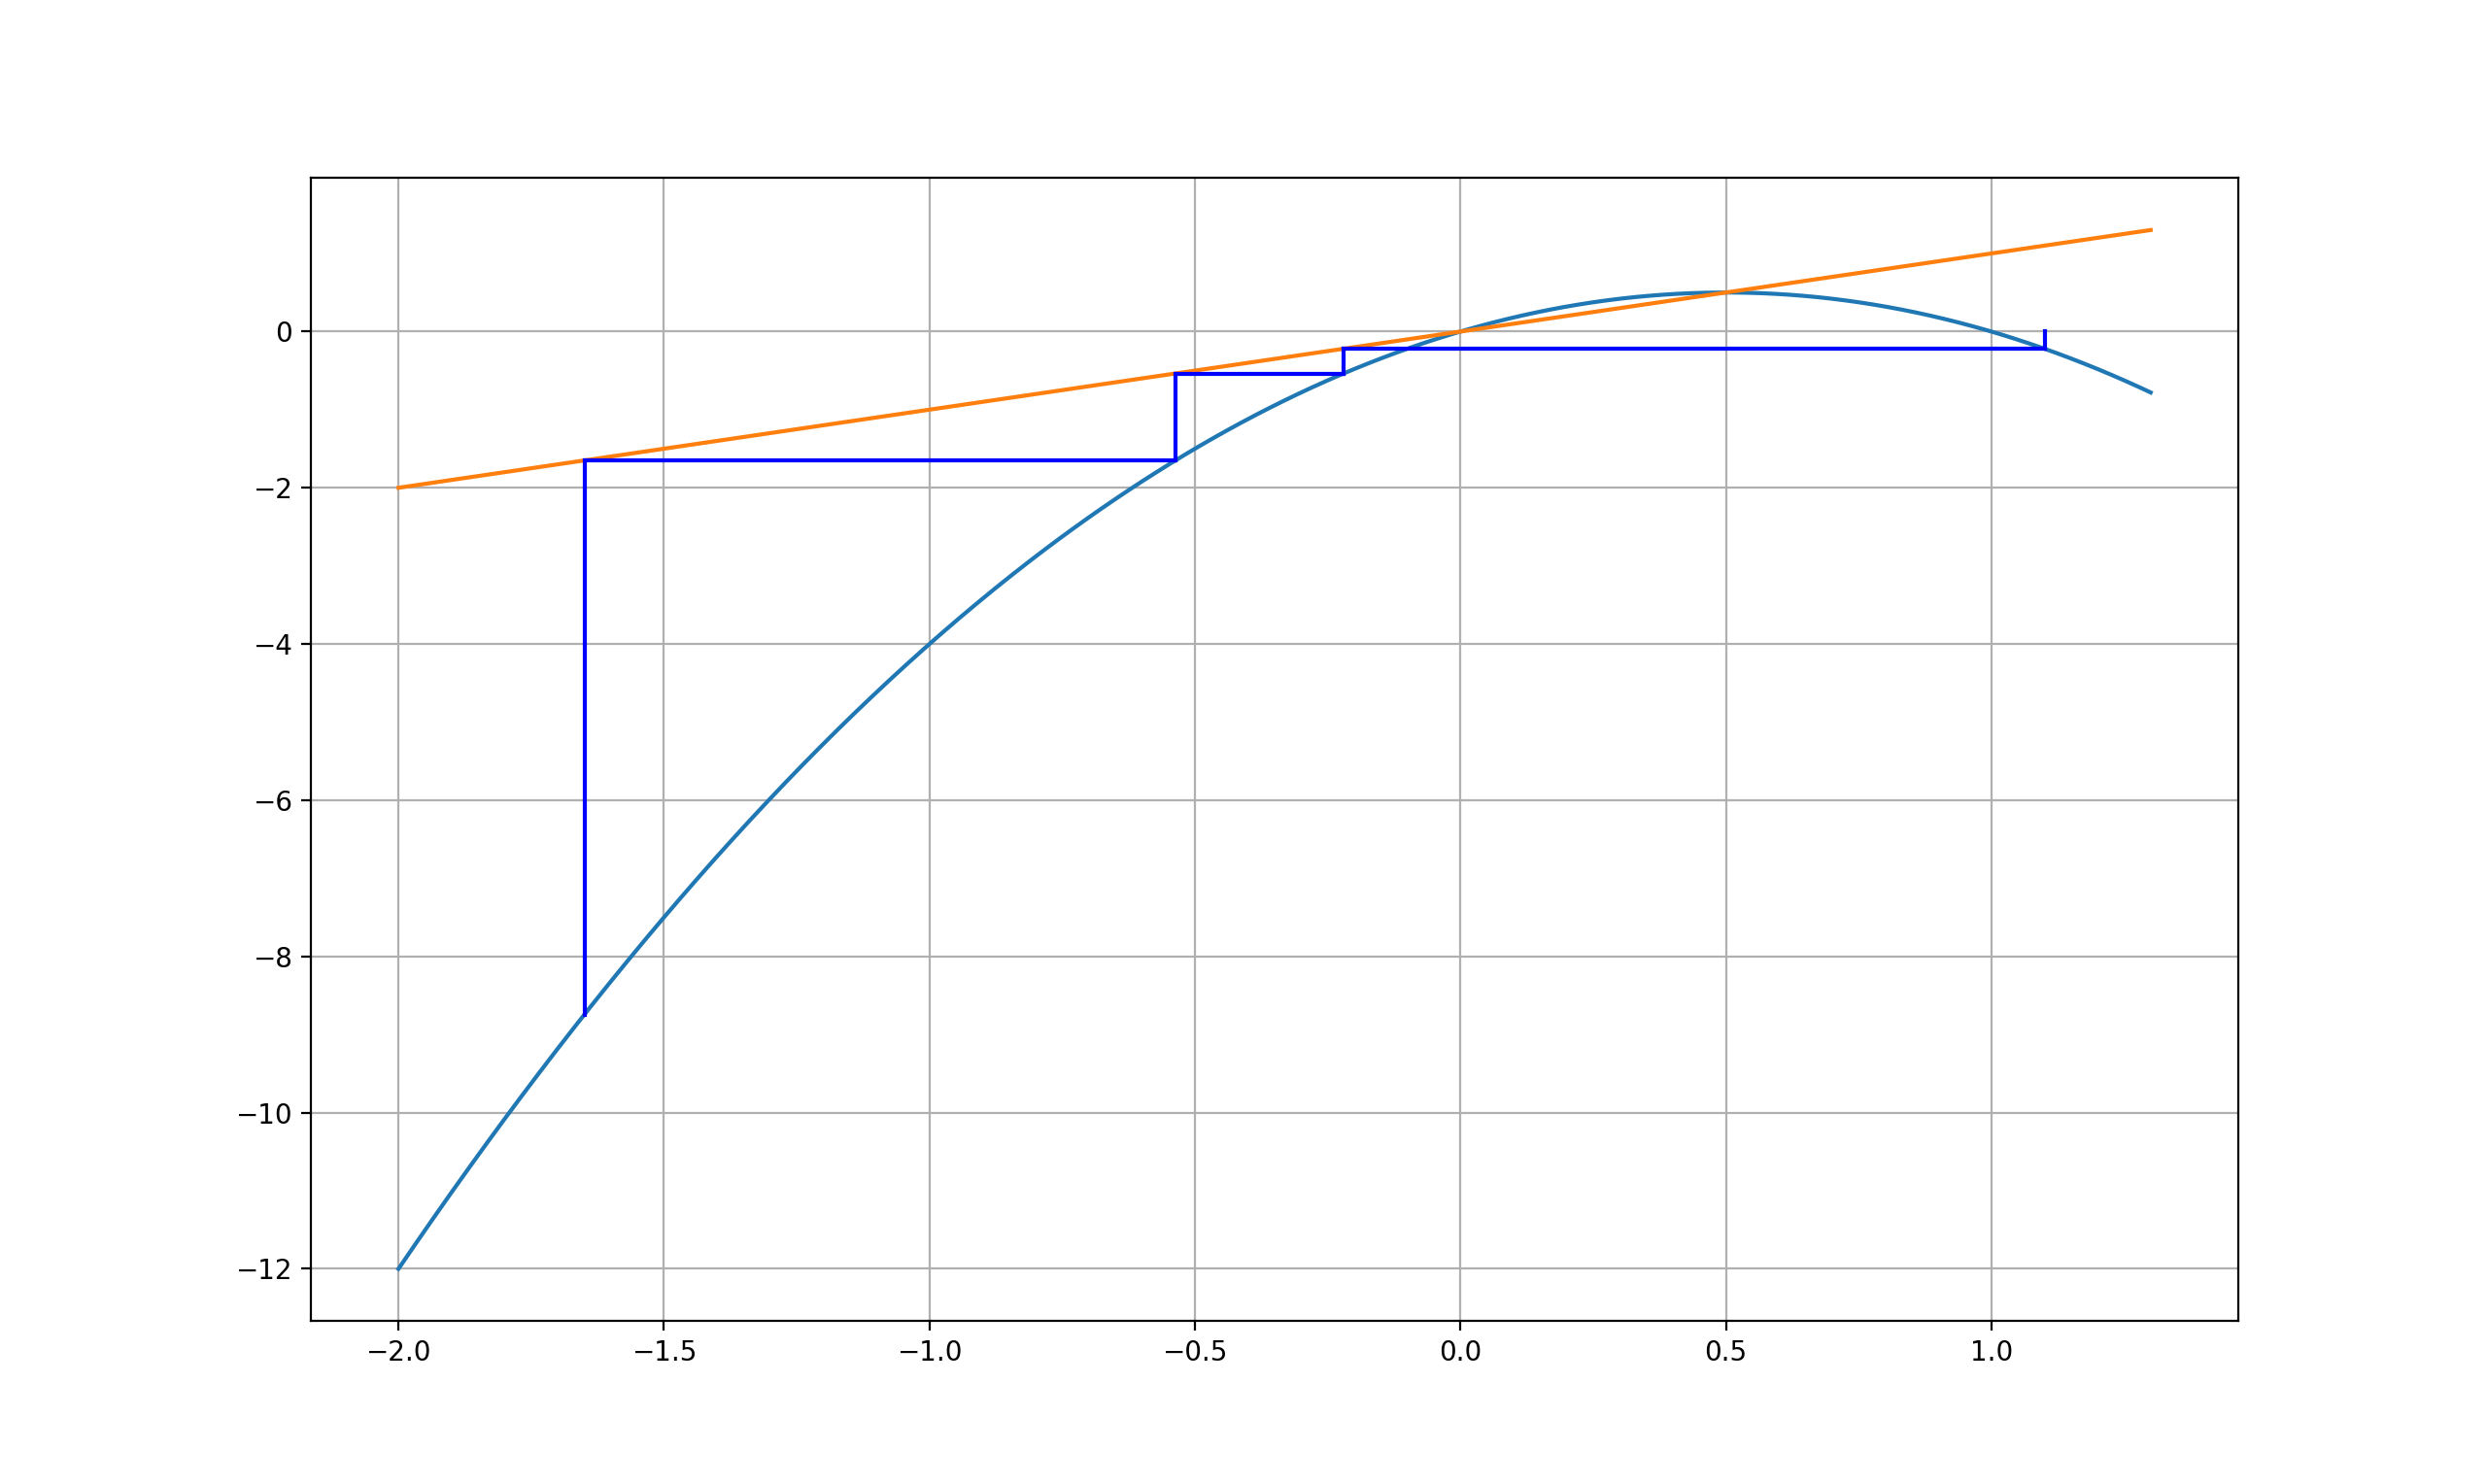
\includegraphics[width=1\textwidth]{figure/section1/cb04.png}
\end{minipage}
\caption{Cobweb plot in different initial value}\label{logistic-cobweb-plot}
\end{figure}


It is simple to find that for all initial value $x \in (0, 1)$, with iteration, the output have limitation in 0.5. On the other hand, to solve the equation $x = 2x(1-x)$ we found $x_1 = 0, x_2 = 1, x_3 = 0.5$ as three fixed point. So we have two kinds of fixed point, the one is limitation point and the other is not.


\begin{definition}\textbf{Sink, Source (Attracting and Repelling Fixed Point)}
\\\noindent Consider a map $f: R \rightarrow R$ and point $p$ s.t. $f(p) = p$, then
\\\noindent If for evert points sufficiently to $p$ are attracted to $p$, then called $p$ as \textbf{sink}, or \textbf{attracting fixed point}. Or
$$
\text{For an } \varepsilon > 0, \forall x \in N_\varepsilon(p), \lim_{k \rightarrow \infty}f^k(x) = p \text{ then called } p \text{ as \textbf{sink}}.
$$
If for every points sufficiently to $p$ are repelled to $p$, then called $p$ as \textbf{source}, or \textbf{repelling fixed point}.
$$
\text{For an } \varepsilon > 0, \forall x \in N_\varepsilon(p), \lim_{k \rightarrow \infty}f^k(x) = p \text{ then called } p \text{ as \textbf{sink}}.
$$
\end{definition}



\newpage

\begin{theorem} \label{sink-source-point}Let $f$ is a map on $R$, assume $p$ is a fixed point of $f$, then
\\\noindent [i] If $|f'(p)| < 1$, then $p$ is a sink;
\\\noindent [ii] If $|f'(p)| > 1$, then $p$ is a source.
\end{theorem}


{\color{blue}
\begin{proof} \textbf{[i]} Based on definition of derivative, we have
$$
\lim_{x \rightarrow p} {|f(x) - f(p)| \over |x - p|} = |f'(p)|
$$
Now. let $a \in (\min(|f'(p)|, 1), \max(|f'(p)|, 1))$ (e.g. $a = {1\over 2}(1+ |f'(p)|)$), then
$$
\forall a \in (\min(|f'(p)|, 1), \max(|f'(p)|, 1)), \exists \varepsilon_0 > 0 \text{ s.t. } \forall \varepsilon \in (0, \varepsilon_0], \forall x \in N_\varepsilon(p), {|f(x) - f(p)| \over |x - p|} < a
$$
            \textit{That means, $f(x)$ is closer to $p$ than $x$ (or distant bewteen curve $y = f(x)$ and $y = x$), but at least a factor of $a$ and we have the conclusion
$$
\forall x \in N_\varepsilon(p), f(x) \in N_\varepsilon(p)
$$
            During the iteration processing it is simple to find that all orbit $\{f(x), f^2(x), \ldots f^n(x), \ldots\} \subset N_\varepsilon(p)$, so now we can consider another conclusion in follow.}
\\[2ex]\noindent \textbf{[ii]} We try to prove the inequality $\forall x \in N_\varepsilon(p), |f^k(x) - p|$
\\\noindent \textbf{[ii-1]} Obvious, if $k = 1$, then $|f(x) - p| = |f(x) - f(p)| < a |x-p|$ ($p$ is fixed point so $f(p) = p$)
\\\noindent \textbf{[ii-2]} If $k = 2$, Based on the conclusion in \textbf{[i]}, $x_1 = f(x) \in N_\varepsilon(p)$ and $|f(x_1) - p| < a |x_1 - p| < a^2 |x - p|$
\\\noindent $\ldots$
\\\noindent \textbf{[ii-k+1]} (Assume the inequality is established in $k$), then
$$
|f^{k+1}(x) - p| < a|f^k(x) - p| < a \cdot a^k |x - p| = a^{k+1}|x - p|
$$
            In summary, for all $k \in N$, the inequality is established.
\\[2ex]\noindent \textbf{[iii-1]} Now we consider the equality condition, if $|f'(p)| < 1$ then $a < 1$ and  
$$
\lim_{k \rightarrow \infty}|f^{k}(x) - p| < |x-p|\lim_{k \rightarrow \infty} a^k = 0 \text{ (Because }a \in (0, 1)\text{)} 
$$
            So we have the conclusion, 
$$
\forall x \in N_\varepsilon(p), \lim_{k \rightarrow \infty}f^k(x) = p
$$
            \textbf{[iii-2]} Also, if $|f'(p)| > 1$ then $a^k \rightarrow \infty$, that means, with the iteration, the maps will eventually outside the condition, or the domain interval. $\blacksquare$
\end{proof}
}

* We will discuss what happened while $f'(p) = 1$ laterly.

** Obviously, this theorem expressed a kind of convergence, as the speed of the convergence is based on the $a$ in exponent function, we called this convergence as \textbf{Exponential Convergence}.

Now we consider another map as example.


\newpage
\begin{example} Solved the fixed point of $\varphi(x) = (3x -x^2)/2$, find every sink and source point with Theo. \ref{sink-source-point}
\end{example}


\begin{figure}[H]
\begin{center}
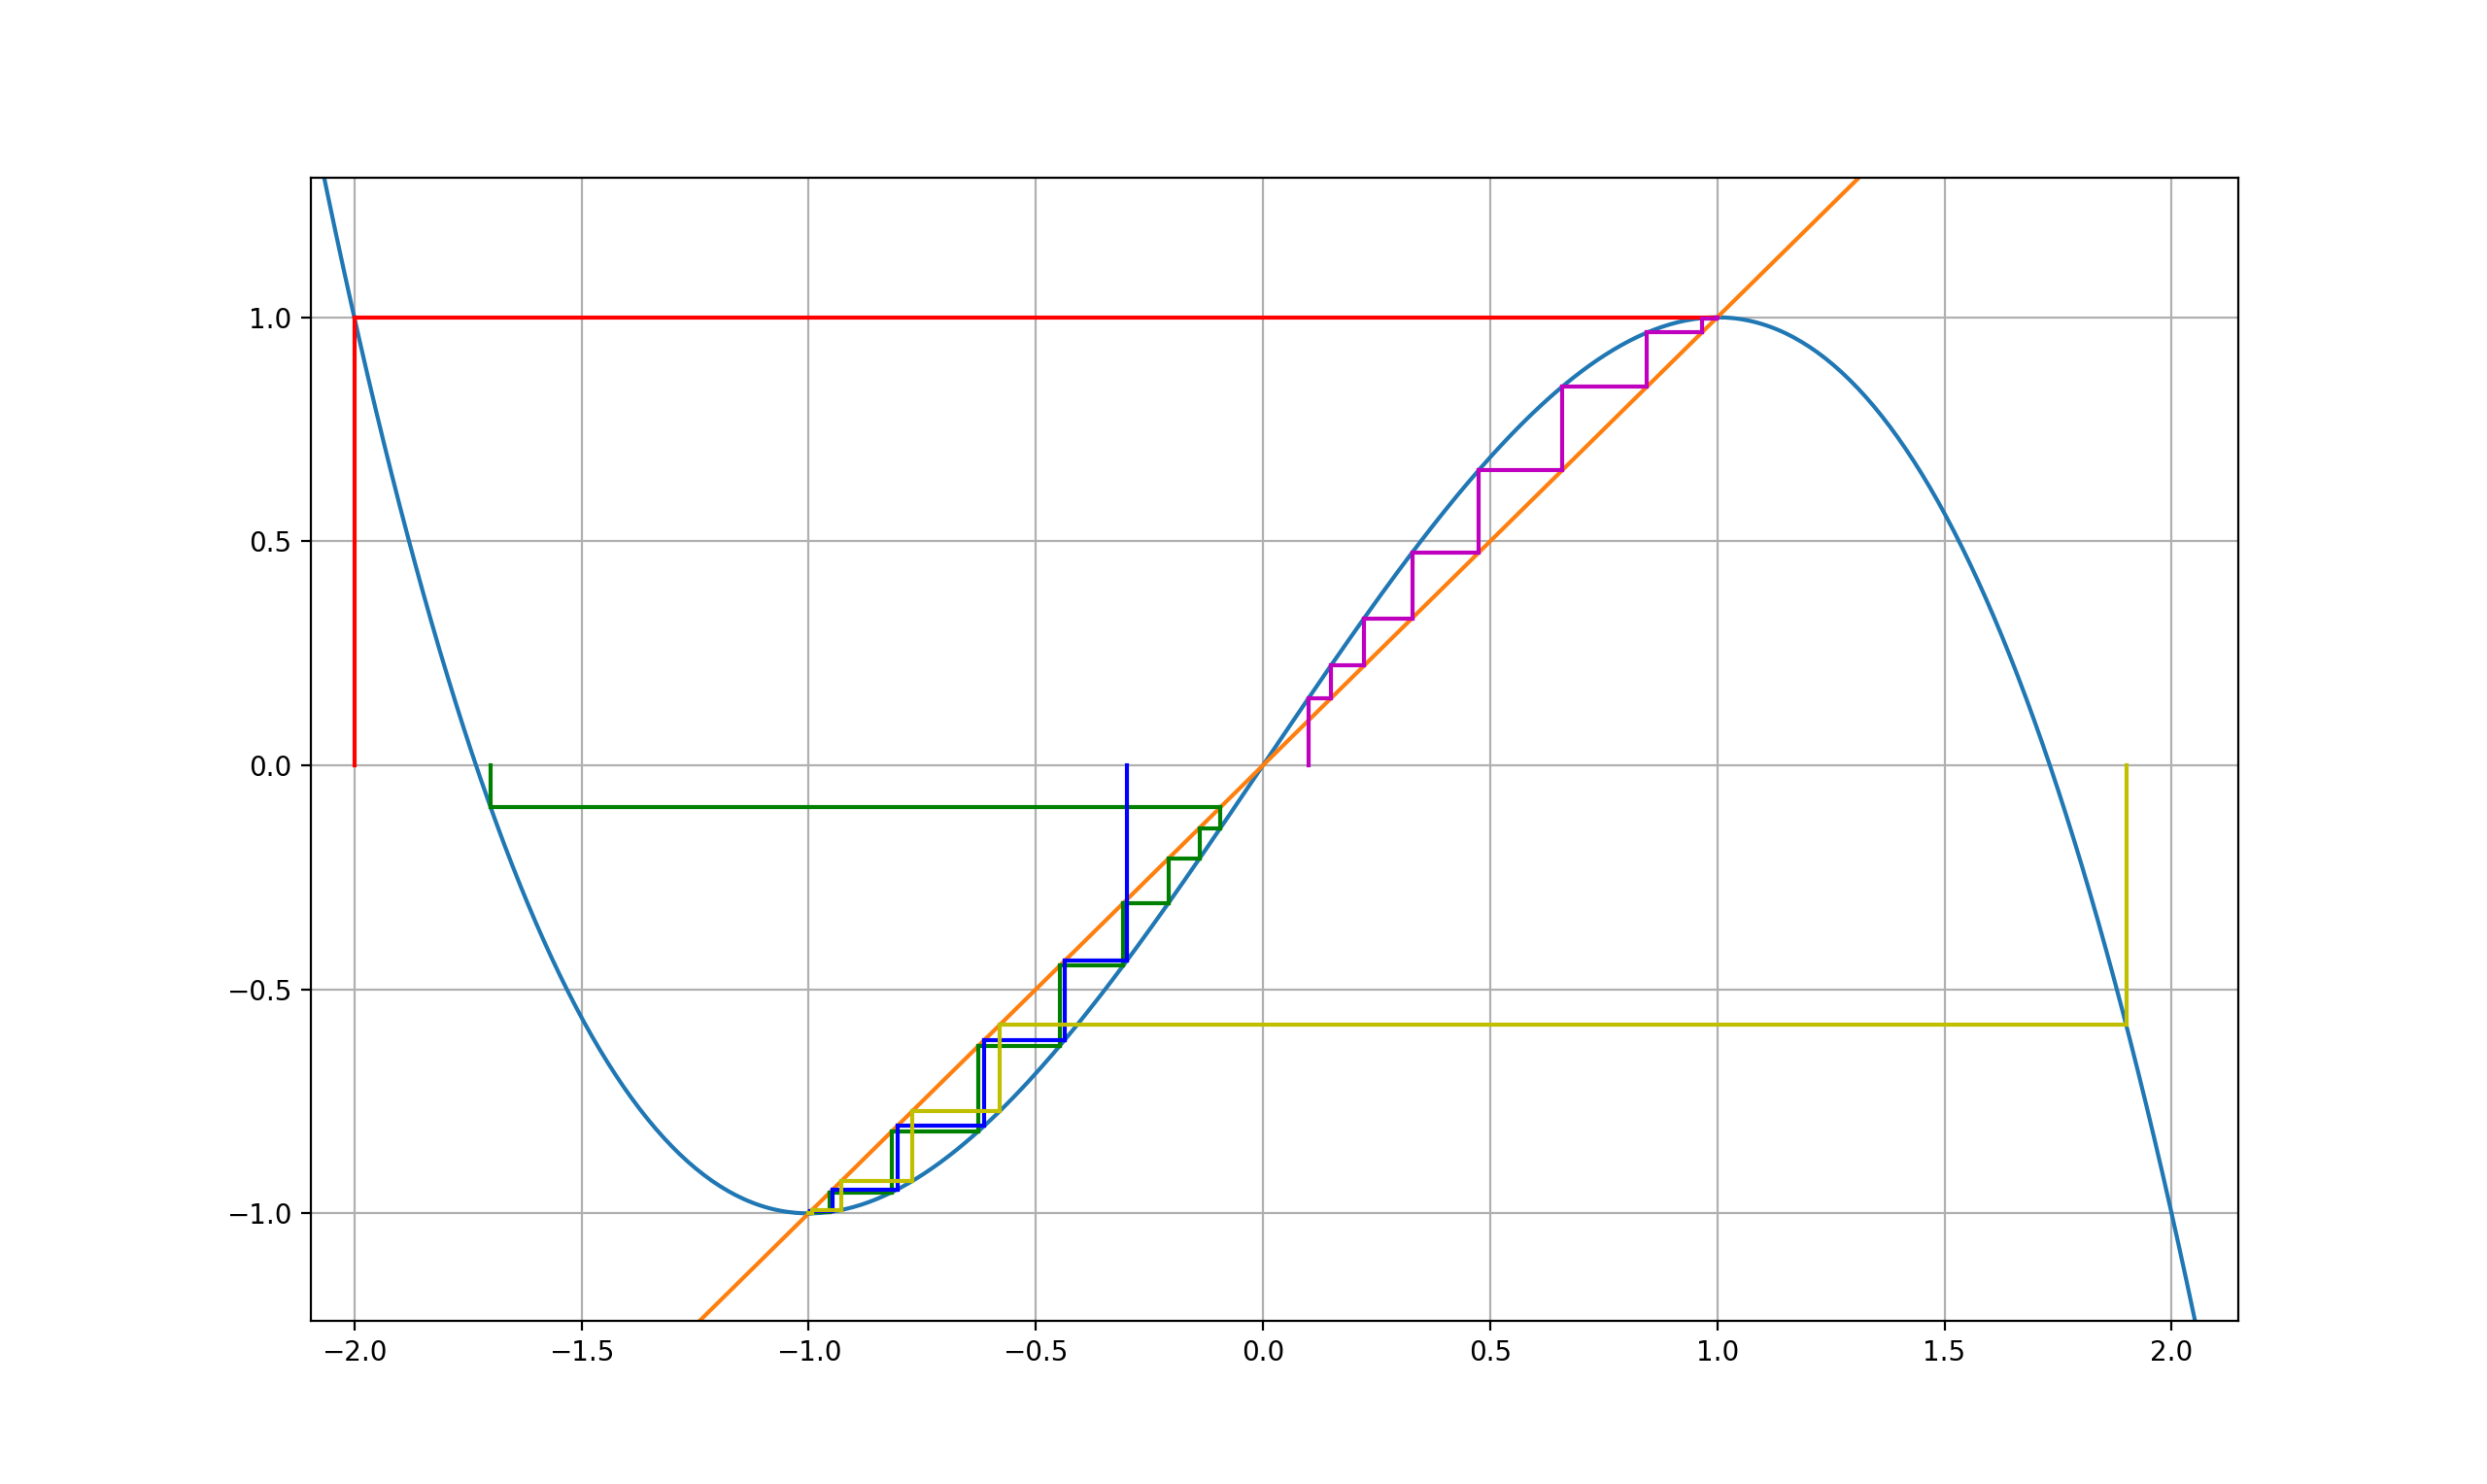
\includegraphics[width=0.5\textwidth]{figure/section1/cobweb-plot-2.png} \\
%\caption{}\label{cobweb-plow-2}
\end{center}
\end{figure}

{\color{blue}
\begin{solution}
It is simple to find the fixed point with $x = (3x - x^3) / 2$ and $x_1 = 1, x_2 = 0, x_3 = -1$. Based on the image, we can found that $1$ and $-1$ are sink and $0$ is source. On the other hand
$$
\varphi'(x) = {3\over 2} (1 - x^2), \varphi'(-1) = 0 < 1, \varphi'(0) = {3 \over 2} > 1, \varphi'(1) = 0 < 1
$$ 
and we proved the conclusion we found on figure before. $\blacksquare$
\end{solution}
}

Another way to confirm a point is sink or source is based on the formula identity and algebra. For instance, we consider the distance bewteen $g(x) = 2x(1-x)$ and fixed point $1/2$, then 
$$
|g(x) - 1/2| = |2x(1-x) - 1/2| = 2|x - 1/2||x - 1/2|
$$

and $\forall x \in (0, 1), |x - 1/2| < 1 \Rightarrow |g(x) - 1/2| < 1$, that means the distance bewteen $g(x)$ and $p$ is decreasing during time iteration and we can confirm that $1/2$ is a sink point rather than source point.

Next, we will focus on a logistic model with different parameter and some property of this new model.


\subsection{Periodic points, family of logistic maps}



\end{document}
%~~~~~~~~~~~~~~~~~~~~~~~~~~~~~~~~~~~~~~~~~~~~~~~~~~~~~~~~~~~~~~~~~~~~~~~~~~~~~~~~~~~~~~~~~~~~~~~~~~~~~






















